\documentclass{beamer}
\usetheme{default}
\setbeamertemplate{navigation symbols}{} % No navigation symbols
\usecolortheme[named=white]{structure} % White titles and such
\setbeamercolor{normal text}{fg=white} % White text
\setbeamercolor{background canvas}{bg=black} % Black background
% Comment this line for default bullet points (triangles)
\setbeamertemplate{itemize item}{\color{white}$\bullet$} 

\begin{document}

\begin{frame}
\end{frame}

\setbeamercolor{background canvas}{bg=white}

\begin{frame}
	\begin{figure}
		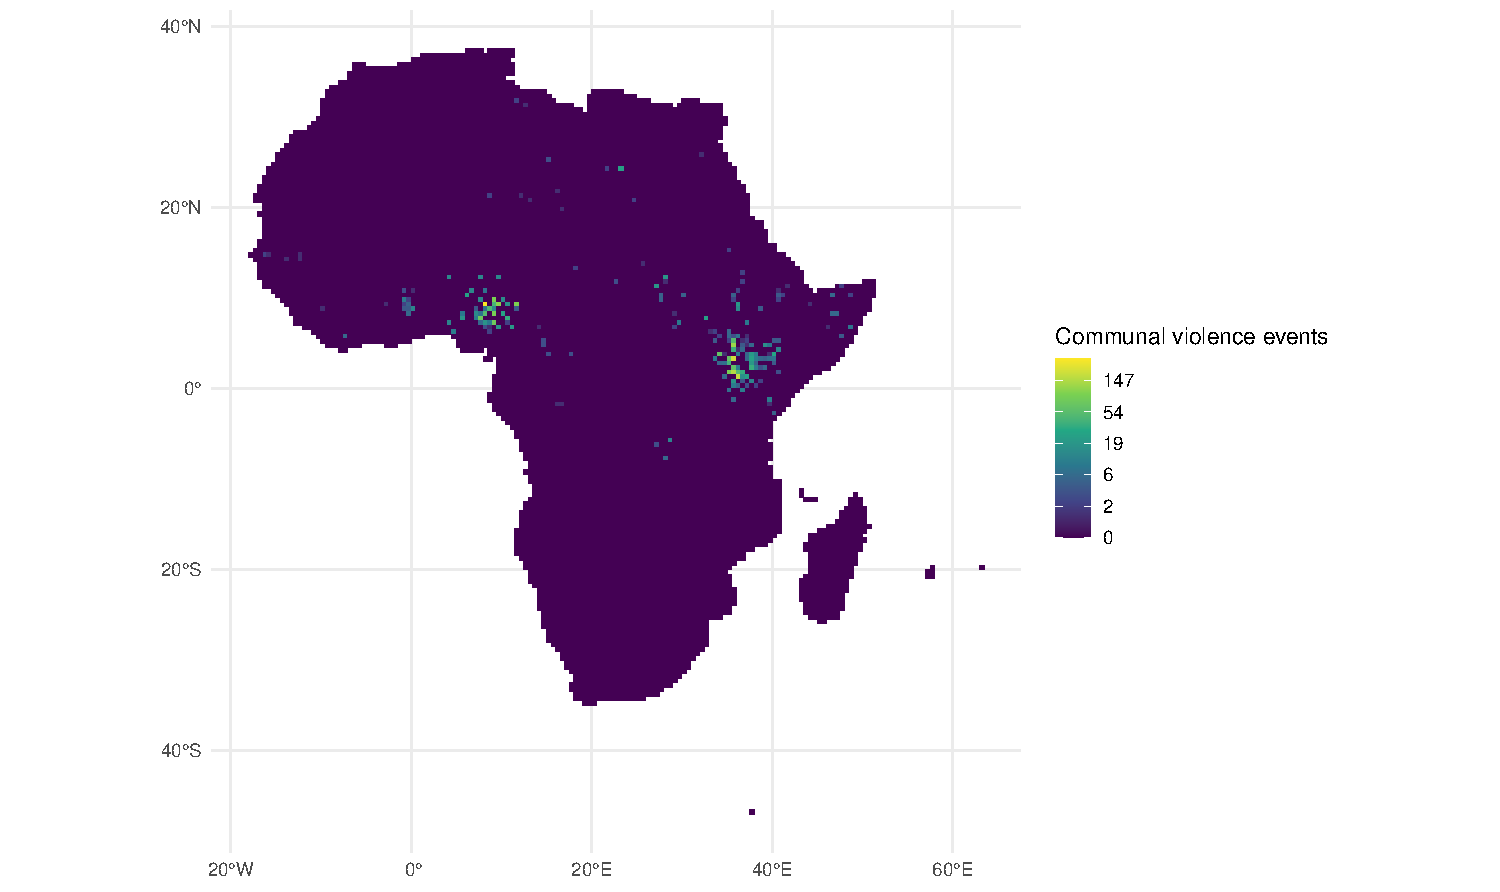
\includegraphics[width=\linewidth]{../R/Output/logOrg3.pdf}
	\end{figure}
\end{frame}

\setbeamercolor{background canvas}{bg=black}

\begin{frame}
\end{frame}

\begin{frame}
	\begin{figure}
		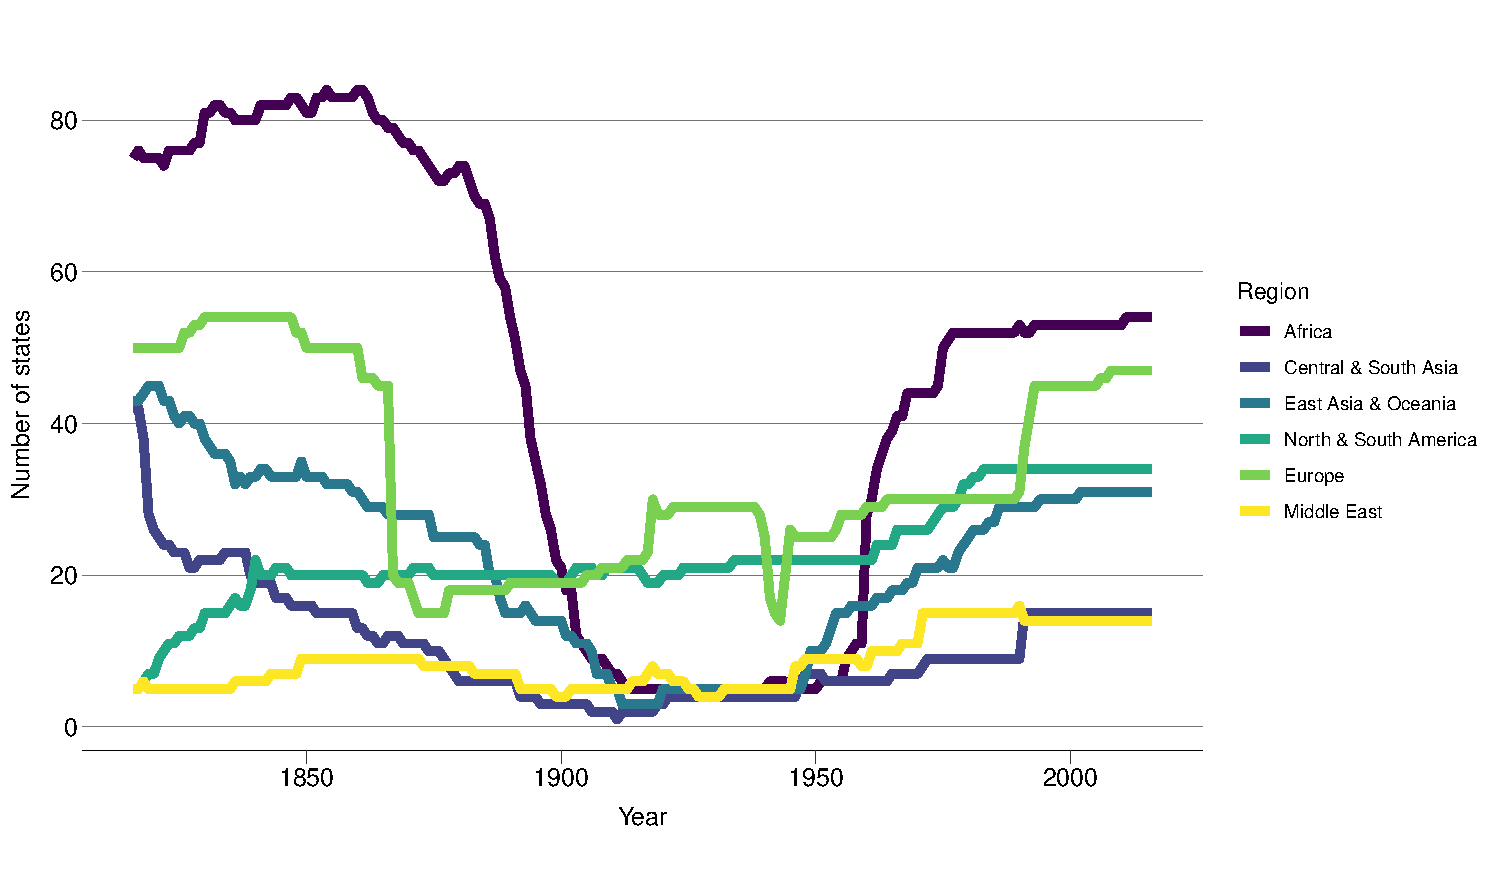
\includegraphics[width=\textwidth]{../R/Output/statesPerYear.pdf}
		\caption{The number of independent states per year.}
		\label{statesperyear}
	\end{figure}
\end{frame}

\setbeamercolor{background canvas}{bg=black}

\begin{frame}
\end{frame}

\setbeamercolor{background canvas}{bg=white}

\begin{frame}
	\begin{figure}
		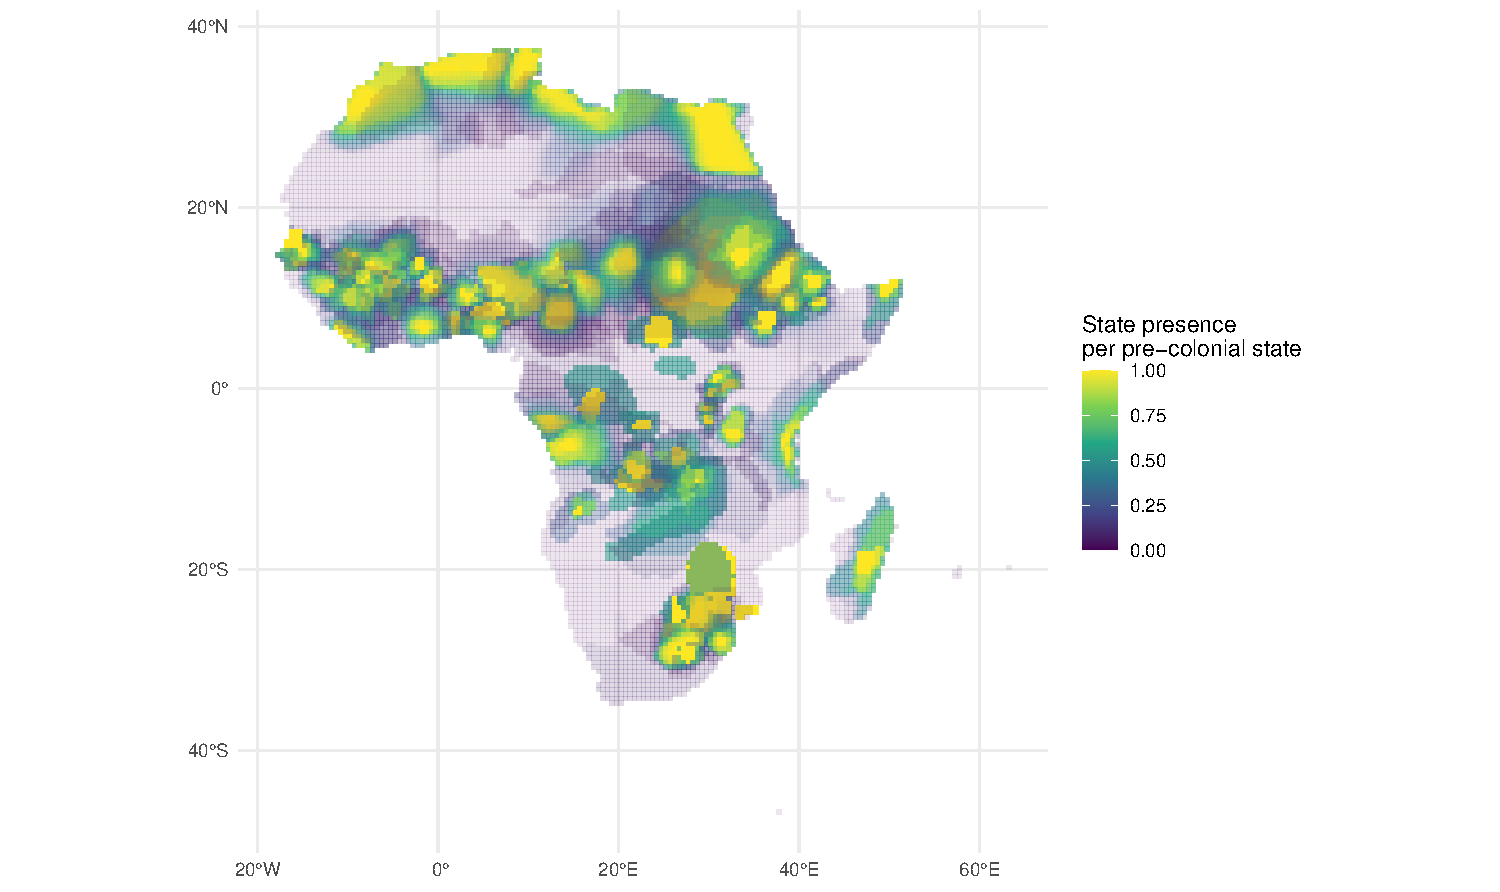
\includegraphics[width=\textwidth]{img/geo_isd_all.pdf}
		\caption{Pre-colonial state presence (normalized per pre-colonial state)}
	\end{figure}

\end{frame}

\setbeamercolor{background canvas}{bg=black}

\begin{frame}
\end{frame}

\setbeamercolor{background canvas}{bg=white}

\begin{frame}
	\begin{figure}
		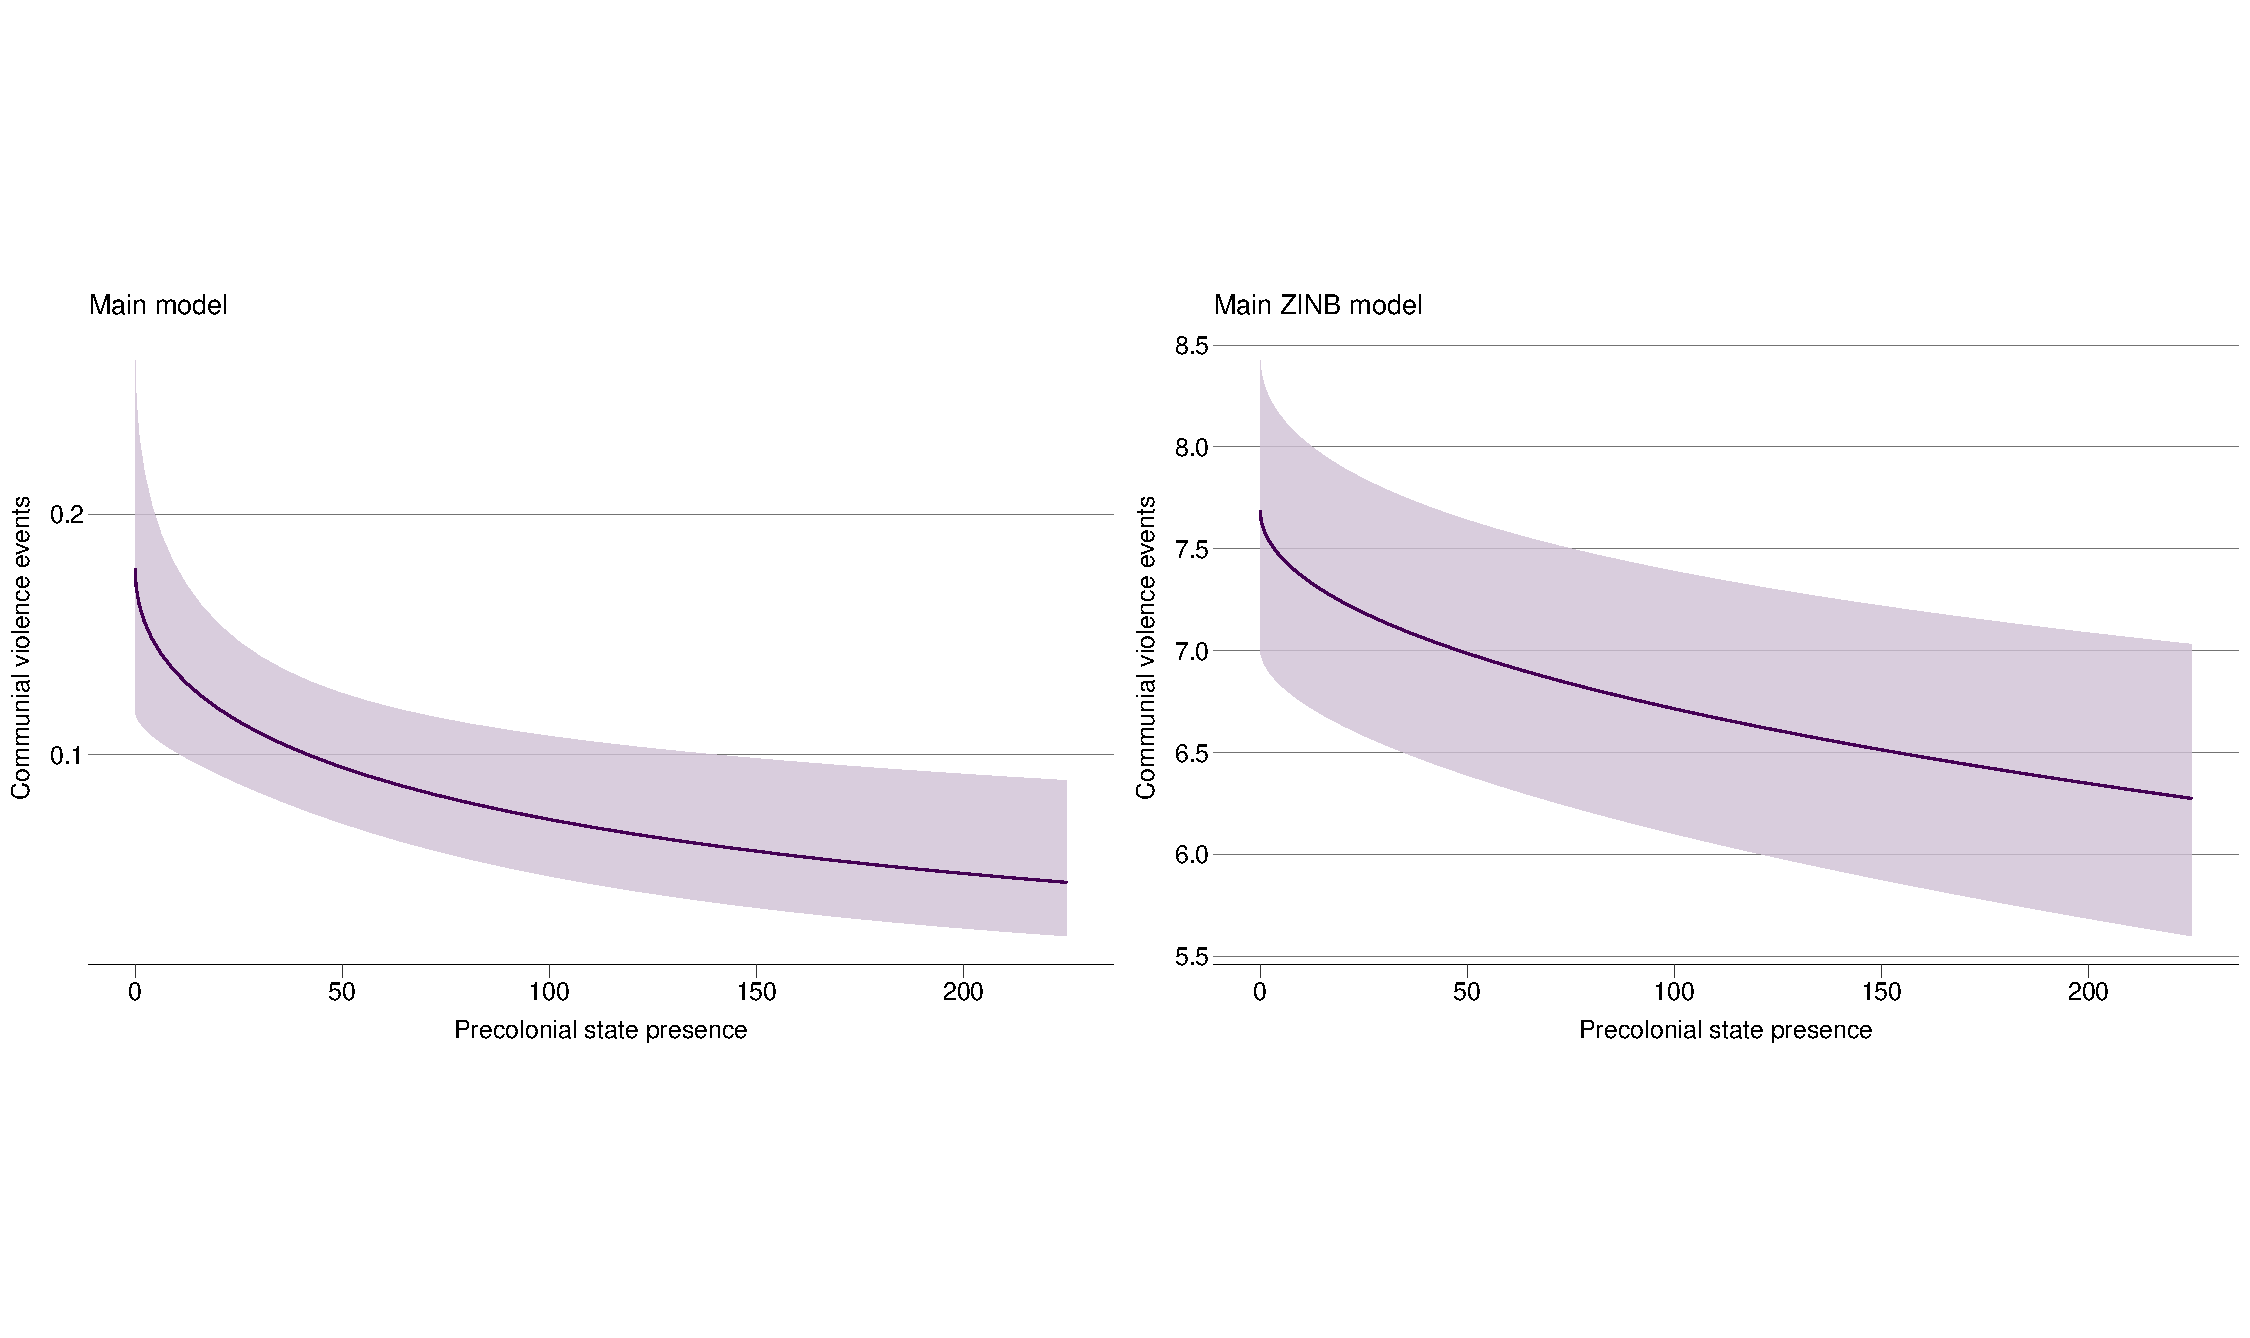
\includegraphics[width=1\linewidth]{R/Output/mainplots.pdf}
	\end{figure}
\end{frame}

\begin{frame}
	\begin{figure}
		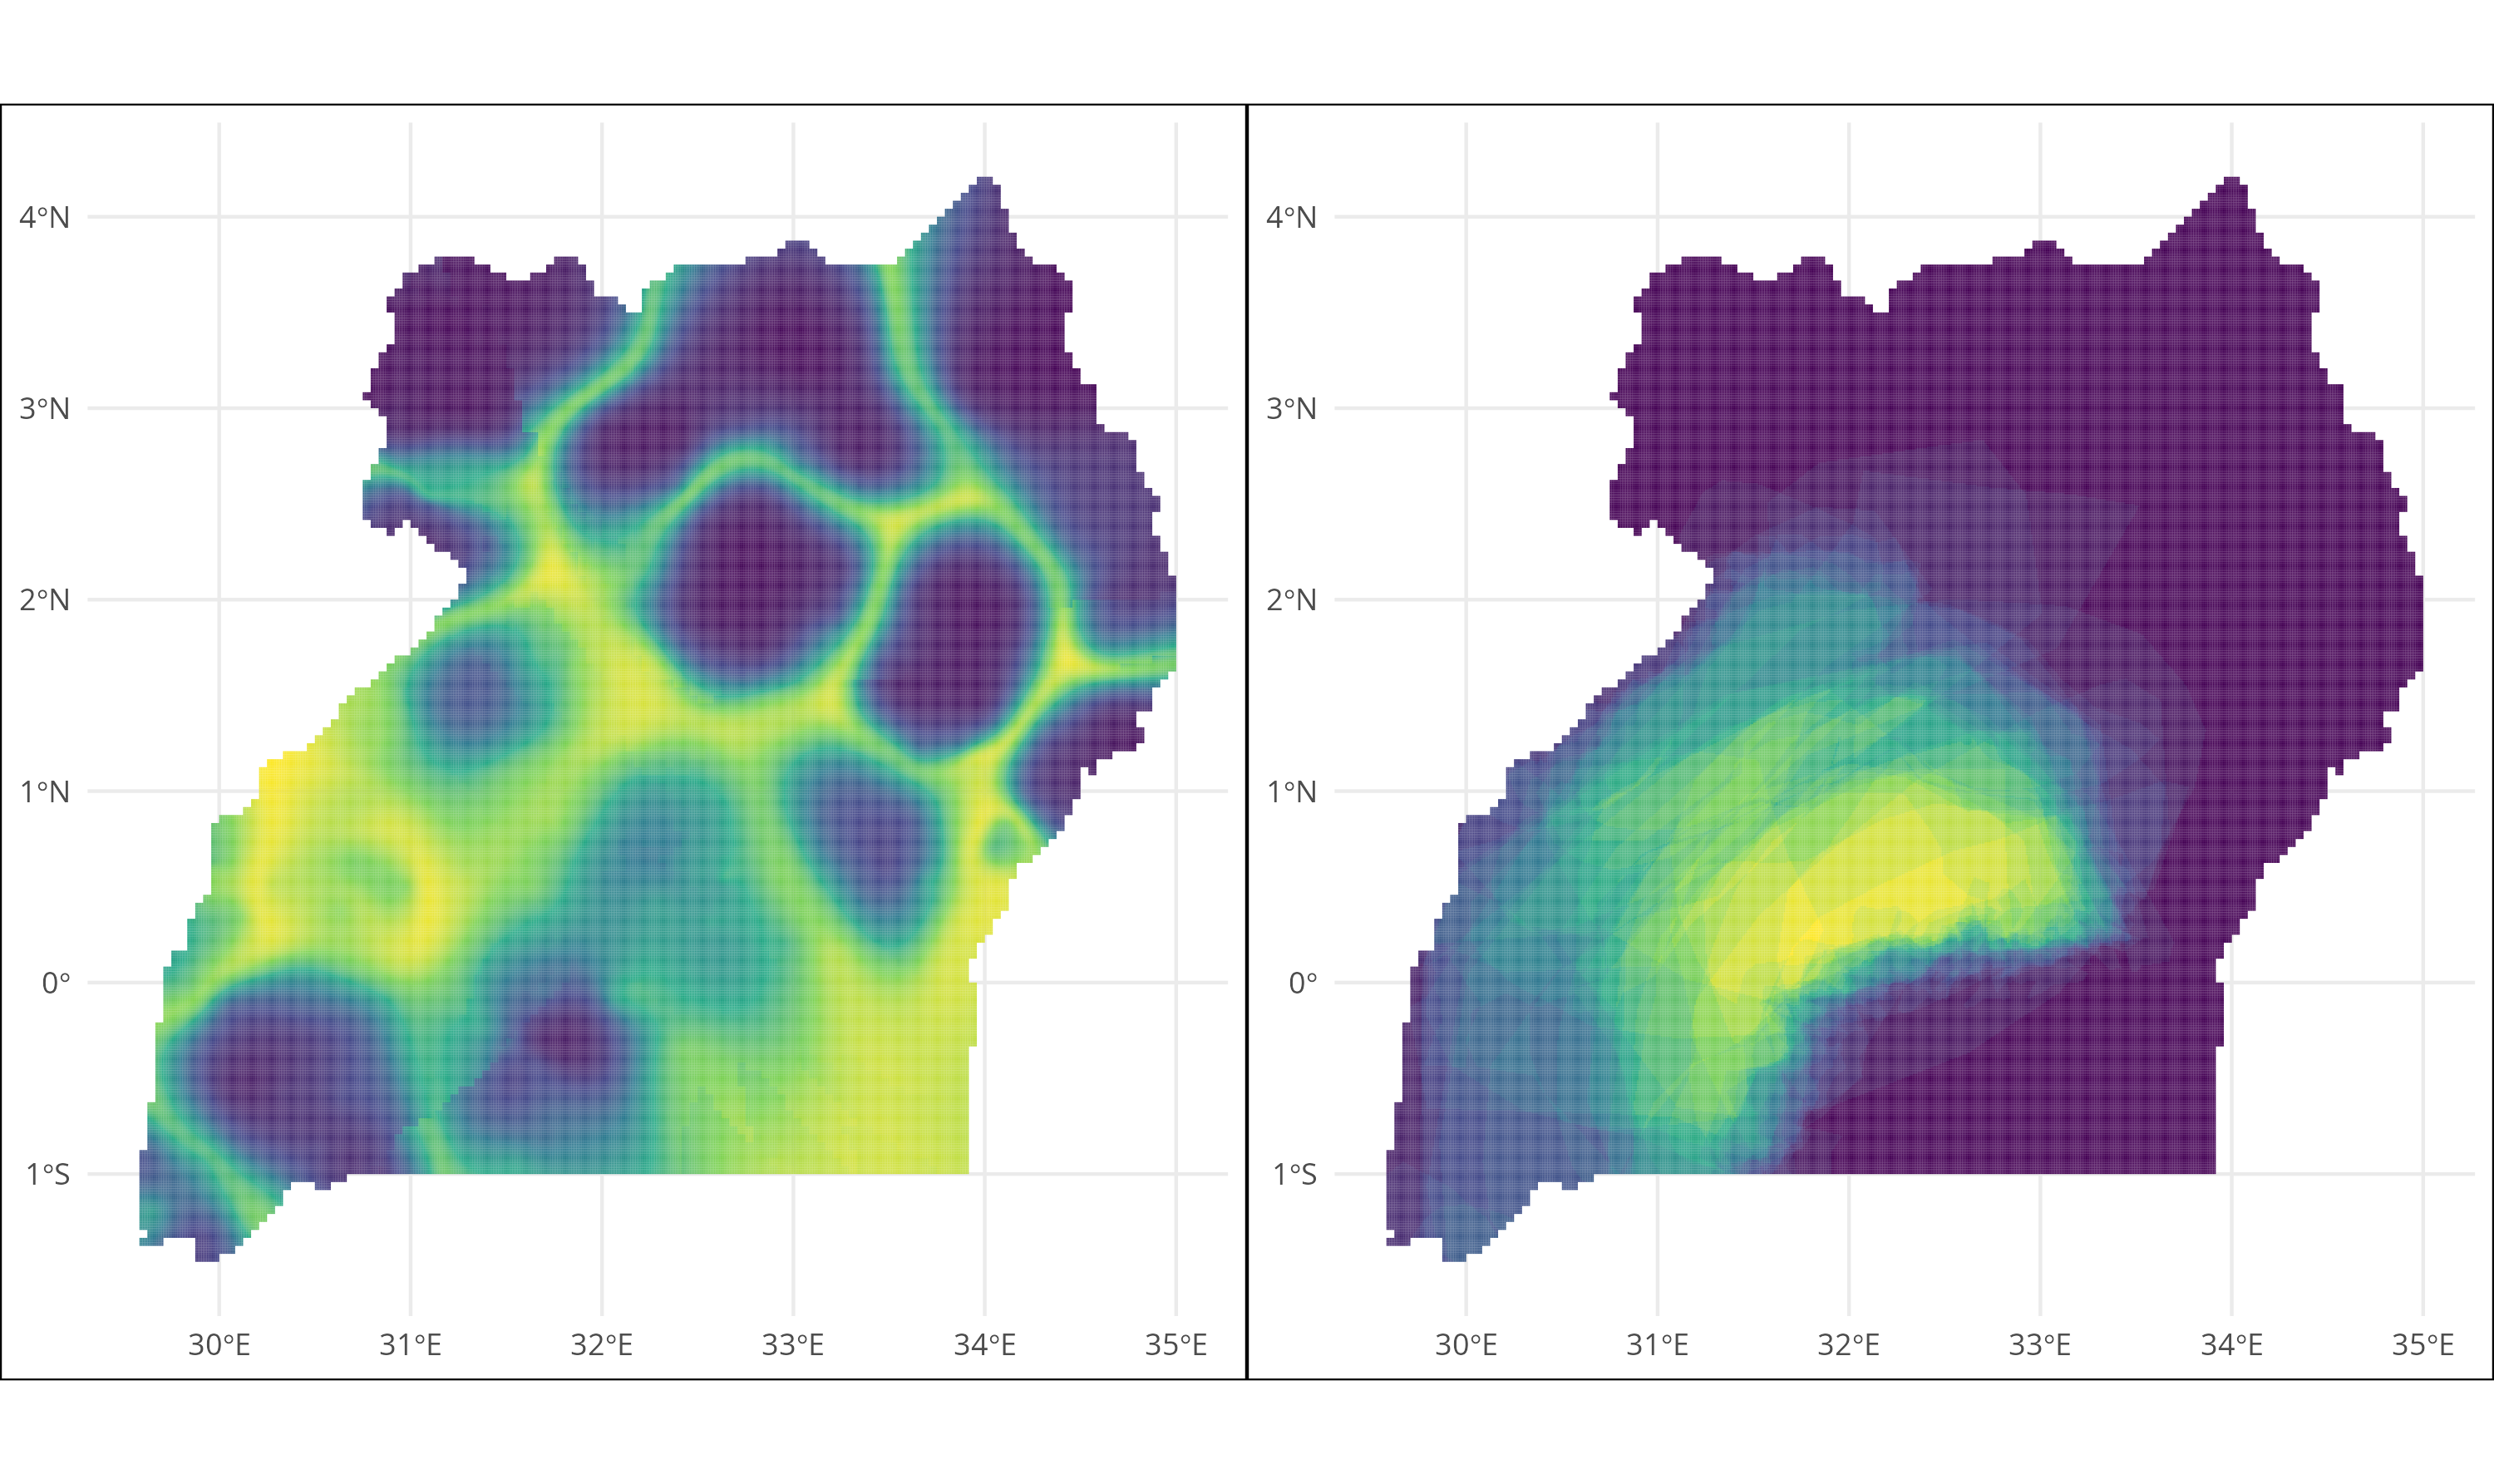
\includegraphics[width=1\linewidth]{img/ugaplots.png}
	\end{figure}
\end{frame}

\end{document}
